\documentclass[11pt, oneside]{article}
\usepackage[a4paper,left=2cm,bottom=2.5cm,right=2cm,top=2.5cm,footskip=1cm]{geometry}
\usepackage{amsmath, amsthm}
\usepackage{amssymb}
\usepackage{verbatim}
\usepackage[export]{adjustbox}
% \usepackage{fontspec}
% \usepackage{fontawesome}
\usepackage{pifont}
\usepackage{array,multirow, rotating}
\usepackage{enumitem}
\usepackage{enotez, multicol}
\setlist[enumerate]{nosep, itemsep=3pt}%, topsep=5pt}
\setlist[itemize]{nosep, itemsep=3pt}%, topsep=5pt}
\renewcommand{\labelitemi}{$\bullet$}
\renewcommand{\theenumiii}{\arabic{enumiii}}
\renewcommand{\labelenumiii}{\theenumiii)}
\usepackage[bottom]{footmisc}
\usepackage{caption, float}
\usepackage{subcaption}
\usepackage{titlesec}
\usepackage{hyperref}
\hypersetup{draft=true}
\usepackage[extrafootnotefeatures]{xepersian}
\twocolumnfootnotes

\newcolumntype{P}[1]{>{\centering\arraybackslash}m{#1}}
\newcolumntype{C}{>{\centering\arraybackslash}c}
\newcolumntype{R}{>{\centering\arraybackslash}r}

\newcommand{\ev}[2]{%
    #1\endnote{
    #1 \hspace*{\fill}  \lr{#2} \hbox to 0.5\textwidth{}
    }
}

\newcommand{\cross}{\ding{53}}
\newcommand{\tick}{\checkmark}
\newcommand{\sel}{\ding{86}}
\newcommand{\ch}{$\bullet$}

\newcommand{\Ms}{\lr{M}}
\newcommand{\Cl}{\lr{C}}
\newcommand{\Vr}{\lr{V}}
\newcommand{\Rc}{\lr{R}}

\newcommand{\Pb}{\lr{P}}
\newcommand{\Dt}{\lr{D}}

\titlespacing*{\subsection}{0pt}{3pt}{0pt}
\titlespacing*{\section}{0pt}{3pt}{0pt}
\titlespacing*{\subsubsection}{0pt}{3pt}{0pt}

\renewcommand\thesection{\arabic{section}-}
\renewcommand\thesubsection{\thesection\arabic{subsection}-}
\renewcommand\thesubsubsection{\thesubsection\arabic{subsubsection}-}

\setenotez{list-name={\raggedleft\rl{واژه‌نامه}}}
\renewcommand\refname{\raggedleft\rl{مراجع}}

% \AtEveryEndnotesList{\begin{multicols}{2}} % before the whole list
% \AfterEveryEndnotesList{\end{multicols}}   % after the whole list
% \AfterEveryListSplit{\begin{multicols}{2}} % after a sub-heading in the splitted list
% \AtEveryListSplit{\end{multicols}}         % before a sub-heading in the splitted list


\setLTRbibitems
\settextfont[
Scale=1.09,
Extension=.ttf,
Path=fonts/,
BoldFont=XB NiloofarBd,
ItalicFont=XB NiloofarIt,
BoldItalicFont=XB NiloofarBdIt
]{XB Niloofar}

\setlatintextfont[Scale=1]{Times New Roman}
\linespread{1.6}
\newtheorem{proposition}{گزاره}
\newtheorem{theory}{قضیه}
\newtheorem{lemma}{لم}
\newtheorem{corollary}{نتیجه}
\newtheorem{system}{سامانه}

% \setlength{\parindent}{0pt}
\setlength{\parskip}{0.4\baselineskip}
\linespread{1.6}

\let\OLDthebibliography\thebibliography
\renewcommand\thebibliography[1]{
	\OLDthebibliography{#1}
	\setlength{\parskip}{0pt}
	\setlength{\itemsep}{0pt plus 0.3ex}
}

% endnote font for persian vocabs
\defpersianfont\multilingual[Scale=0.9, Extension=.ttf, Path=fonts/]{XB Niloofar}

\DeclareInstance{enotez-list}{custom}{paragraph}
{
notes-sep = -7pt,
format =  \multilingual,
number = \begin{persian} \rl{#1}\end{persian}.
}

\def\enoteformat{\rightskip=0pt \leftskip=0pt \parindent=0.5em \leavevmode\llap{\makeenmark}}



\pagenumbering{gobble}
\begin{document}
	\begin{titlepage}
		\linespread{1.5}
%		\settextfont[Scale=1.2]{B Yas}
%		\setlatintextfont[Scale=1.0]{Times New Roman}
		\centering
		
\includegraphics[width=3cm]{sharif-logo.png}\\[\bigskipamount]
		\normalsize	\textbf{دانشگاه صنعتی شریف}\\
		\textbf{دانشکده مهندسی کامپیوتر}\\
		\textbf{سمینار کارشناسی ارشد گرایش نرم‌افزار}%
		\\[1.3cm]

		{\LARGE		عنوان:\\
		\textbf{تحلیل صف‌بندی گروه‌های نظیر به نظیر}\\
		\textbf{\lr{Queueing analysis of peer-to-peer swarms}}\\[2cm]}

		{\Large
		\textbf{نگارش:} \\
		امیر امیری\\
		400202020\\[1.3cm]
		\textbf{استاد راهنما:} \\
		جناب آقای دکتر حسین حسینی\\[1.3cm]

		\textbf{استاد ممتحن داخلی:}\\
		جناب آقای دکتر محمد محمدی\\[1.3cm]
		\vfill
		\textbf{بهمن 1401}
		}
	\end{titlepage}
	\clearpage
	\pagenumbering{arabic}
	\setcounter{figure}{0}
	\newgeometry{margin=2cm, bottom=2cm}


\section*{چکیده}
‫این مقاله به بررسی پویایی‌ تبادل فایل نظیر به نظیر از دیدگاه صف‌بندی می‌پردازد. در این سامانه‌ها، نرخ سرویسی که یک نظیر دریافت می‌کند  دو چیز، یکی به یک کامپوننت (مانند کارگزاران یا سیدر‌ها) غالبا ثابت و دیگری تعداد نظیرهای حاضر در عملیات وابسته است. این پژوهش یک کلاس از صف‌های $M/G$ اشتراک پردازنده تحلیل شده است که جمعیت و بار کاری باقی‌مانده در این شرایط را توصیف می‌کند و مشخصه‌های عامل ایستای ‌آن را در حالت تعداد کارگزاران ثابت برمی‌شمریم و نشان می‌دهیم نتیجه مانند ترکیب دو صف از نوع $M/G/1$ و $M/G/\infty$ است. حدهای مقیاسی بر روی این صف اعمال شده و دو عامل محدودکننده، وابسته به اینکه مشارکت کارگزار یا نظیر تبدیل به مشارکت غالب می‌شود را شناسایی شده است. همچنین حالتی که تغییر آرام گوناگونی جمعیت کارگزاران اتفاق می‌افتد نیز با بسط دادن مورد از طریق تحلیل‌ شبه-ایستا نیز بررسی شده است.
\\[1ex]
\textbf{کلمات کلیدی}: نظیر به نظیر، صف‌های اشتراک پردازنده، اندا‌زه‌های عمومی، حد‌های سیال


\section{مقدمه}
‫در سالیان اخیر، استفاده سامانه‌های به اشتراک گذاری فایل نظیر به نظیر مانند
\ev{بیت‌تورنت}{‌Bittorent}
\cite{c1}
‫گسترده شده است و بخش مهمی از ترافیک اینترنت را به خود اختصاص داده است. محتوا با تقسیم به قطعه‌های کوچک (تکه)
‫منتشر می‌شود و نظیر را قادر به تبادل این واحدها را به صورت دو طرفه می‌سازد. قدرت نظیر به نظیر از معنی توزیع محتوا بر روی حقیقتی استوار است که نظیرهای در حال بارگیری، همزمان مشغول به بارگذاری تکه‌ها برای بقیه هستند؛ بنابراین عرضه ظرفیت خدمت برای یک محتوای معین با تقاضای متناظر مقیاس می‌گیرد.


‫مجموعه نظیرها یک فایل محتوایی مشخصی که اغلب با عنوان
\ev{گروه}{Swarm}
‫از آن یاد می‌شود با یکدیگر تبادل می‌کنند که در هر کدام دو کلاس مشخص است؛ تعدادی نظیر (در ادبیات بیت‌تورنتی،
\ev{سیدر}{Seeder}
‫ها) که در حال حاضر همه فایل را در اختیار دارند و به مانند کارگزار برای سایرین عمل می‌کنند، در حالی که نظیرهای در حال بارگیری
(\ev{لیچر}{Leecher})
‫همزمان نقش کارخواه و کارگزار را ایفا می‌کنند. این گروه‌ها در طی زمان و بر اساس رسیدن‌ها و خروج‌های نظیرها تکامل می‌یابد؛ بنابراین عادی است که پویایی جمعیت‌ آنها را با ابزارهای فرضیه صف‌بندی تحلیل و بررسی کرد.
‫
\begin{proposition}
‫اگر داشته باشیم $\rho:=\lambda/\mu$، توزیع آرامش برای تعداد لیچرها در فرآیند تولد-مرگ (1) به صورت زیر است:

\begin{equation}
\pi(n)=\pi(0)\prod_{i=1}^{n}\frac{\lambda}{\mu (i+y_0)}=\left[\sum_{m=y_0}^{\infty}\frac{\rho^m}{m!}\right]^{-1}\ \frac{\rho^{n+y_0}}{(n+y_0)!}\quad for\ n \geq 0
\end{equation}
\end{proposition}

‫به طور خاص، سامانه برای هر $\lambda$، $\mu$ و $y_0$ پایدار است.

‫توجه داشته باشید که این سامانه می‌تواند به عنوان ترکیبی از صف‌های $M/M/1$ و $M/M/\infty$ دیده شود. اگر از مشارکت لیچرها صرف نظر کنیم، این سامانه به یک صف $M/M/1$ با بار $\lambda/(\mu y_0)$ تقلیل می‌یابد و تنها برای $\rho<y_0$ که به دلیل مقابله تنهای سیدرها با بار سامانه طبیعی است، پایدار خواهد بود. اگر مشارکت سیدرها صرف نظر کنیم، سامانه به یک صف $M/M/\infty$ تبدیل می‌شود و سامانه برای تمام مقادیر $\rho$ پایدار خواهد بود. در حالت $\rho>y_0$ نیز مشارکت لیچرها برای حفظ پایداری لازم خواهد بود.


‫برای تحلیل‌های بیشتر این سنجه‌های تصادفی، یک توصیف مشخصه متقاعد کننده تابع لاپلاس است که به این صورت تعریف می‌شود:


\begin{equation*}
\mathcal{L}_\Phi\left[f\right]=E\left[e^{-\int_{0}^{\infty}f(\sigma)\Phi(d\sigma)}\right]
\end{equation*}


‫که برای هر $f\geq0$ و محدود به $\mathbb{R}^+$ برقرار خواهد بود. حالا این تابع را بر روی توزیع غیرمتغیرمان که تعریف کردیم اعمال می‌کنیم.

\begin{proposition}
‫توزیع ایستای فرآیند $\Phi_t$، یک سنجه تصادفی در $\mathbb{R}^+$ با تابع لاپلاس:
\begin{equation}
\mathcal{L}_\Phi\left[f\right]=G\left(\int_{0}^{\infty}e^{-f(\sigma)}\bar{H}(d\sigma)\right)
\end{equation}
‫است که برای هر $f\geq0$ که $G(.)$ یک $pgf$ از $\pi$ است برقرار خواهد بود.
\end{proposition}

\begin{equation}
\mathcal{L}_\Phi\left[f\right]=\int_{n=0}^{\infty}E\left[e^{-\int_{0}^{\infty}f(\sigma)\Phi(d\sigma)}\ |\ x=n\right]\pi(n)
\end{equation}


‫نرخ‌های گذار زنجیره مارکو
‫ $(x(t),y(t))$ که در سامانه در شکل \ref{fig:1} تعریف شده‌اند به صورت زیر است:
‫

\begin{subequations}
\begin{align}
q_{(x,y),(x+1,y)}&=\lambda,\\
q_{(x,y),(x-1,y+1)}&=\alpha\mu(x+y)1_{\{x>0\}},\\
q_{(x,y),(x-1,y)}&=(1-\alpha)\mu(x+y)1_{\{x>0\}},\\
q_{(x,y),(x,y-1)}&=\gamma y
\end{align}
\end{subequations}


\begin{figure}[!ht]
	\centering
	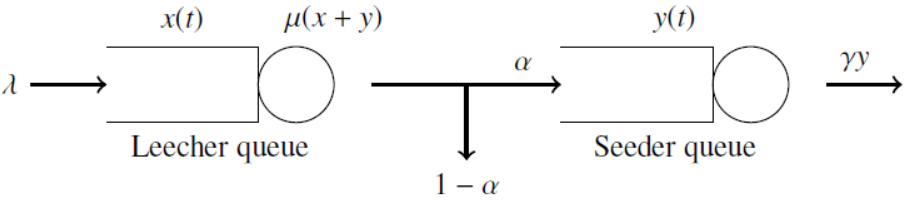
\includegraphics[width=0.8\columnwidth]{resources/fig1.png}
	\caption{صف‌بندی شبکه برای تحلیل شبه-ایستا}
	\label{fig:1}
\end{figure}

‫با مفروضات بالا، $\alpha$ و $\gamma$ کوچک خواهند شد و دومین صف در مقیاس زمانی بزرگتری نسبت به صف اول فعالیت خواهد کرد. نشان می‌دهیم که تحت یک حد مناسب، تحلیل سامانه ترکیبی به این دو مقیاس زمانی تقسیم می‌شود.
در اینجا یه کلمه بزرگتر را برای واژه نامه تست می‌کنیم، این کلمه
\ev{شناساگر موجودیت نامگذاری شده}{Named Entity Recognizer}
است.


\begin{figure}[!ht]
	\centering
	\begin{subfigure}[b]{0.5\columnwidth}
		\centering
		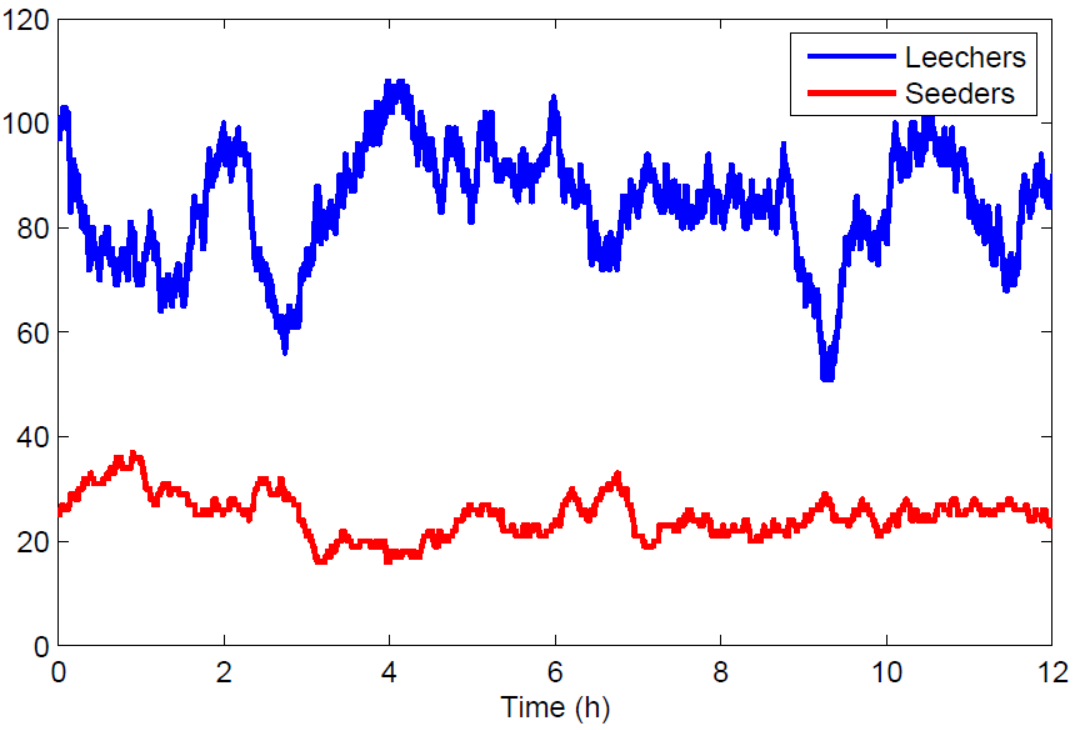
\includegraphics[width=0.8\columnwidth]{resources/fig4_a.png}
		\caption{نکامل تعداد لیچرها در زمان (بالایی)}
	\end{subfigure}\hfill
	\begin{subfigure}[b]{0.5\columnwidth}
		\centering
		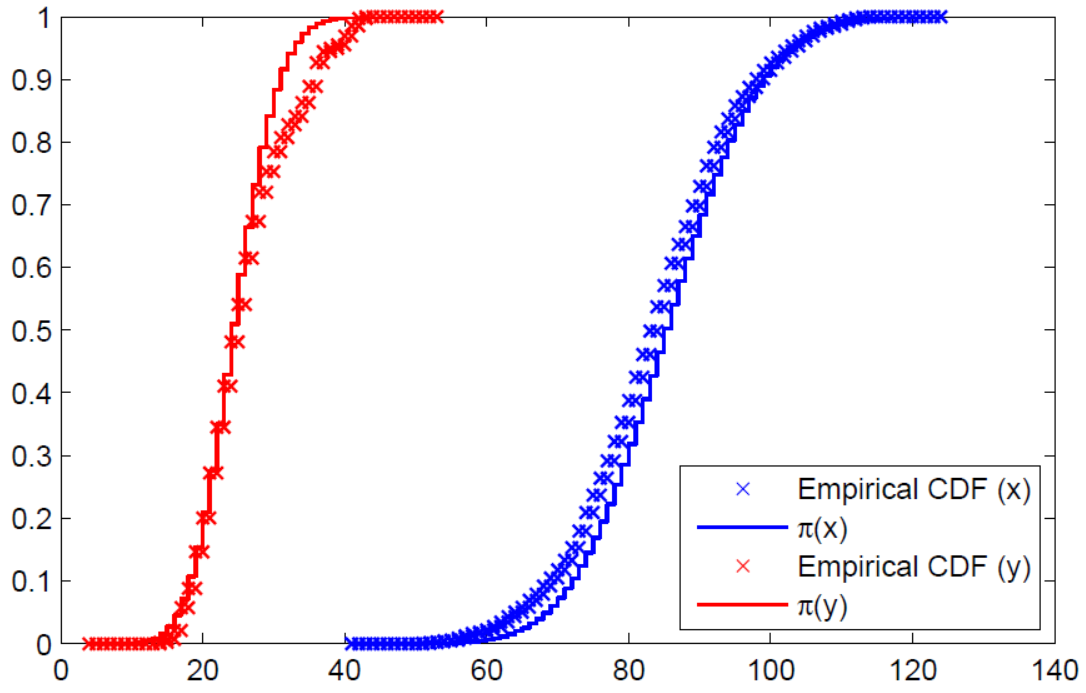
\includegraphics[width=0.8\columnwidth]{resources/fig4_b.png}
		\caption{توزیع حالت سکون تکامل تعداد لیچرها (پایینی)}
	\end{subfigure}
	\caption{نتایج شبیه‌سازی برای حالت $\rho>y_0$}
\end{figure}



\section{نتیجه‌گیری}

‫در این مقاله، یک مدل صف‌بندی برای شبکه تبادل فایل نظیر به نظیر را تحلیل کردیم. ما به طور خاص بر روی سامانه‌ای با تعداد ثابتی سیدر تمرکز کردیم که به ما امکان پیشرفت در تحلیل از دیدگاه صف‌بندی با توجه به مدل‌های قبلی را داد. ما یک کلاس از صف‌های اشتراک پردازنده $M/G$‌ قابل ردگیری  شناسایی کردیم، شخصات توزیع ایستایشان را نیز مشخص کردیم و نشان دادیم که به اندازه‌های کار غیرحساس است؛ بنابراین برای کارهای غیرقطعی سامانه‌های نظیر به نظیر مناسب هستند. ما همچنین سامانه را تحت یک شبکه بزرگ تقریبی تحلیل کردیم و نشان دادیم که می‌تواند توسط یک صف $M/G/1$ یا یک صف انتقال داده شده $M/G/\infty$ وابسته به مغلوب بودن مشارکت کارگزار و یا نظیر، تقریب زده شود. در نهایت ما نتایج را برای سیدرهای ثابت به حالتی که جمعیت سیدرها به آرامی تغییر می‌کند تعمیم دادیم. تمام نتایج با شبیه‌سازی‌های سطح بسته به طور دقیق اعتبارسنجی شدند.


\linespread{1.0}
\latinfont
\bibliographystyle{ieeetr}
\bibliography{seminar}
\printendnotes[custom]

\end{document}
